\documentclass[9pt]{beamer}

%!TEX root = ../notas_de_clase.tex

%preamble

%language
\usepackage[spanish,es-nodecimaldot]{babel}
\usepackage[utf8]{inputenc}
\usepackage{apacite}
\usepackage[absolute,overlay]{textpos}

%packages
\usepackage[Algoritmo]{algorithm}
\usepackage{algorithmicx}
\usepackage[noend]{algpseudocode}
\usepackage{mathtools}
\setlength {\marginparwidth}{2cm}
\usepackage{todonotes}
\usepackage{amsbsy}
\usepackage{amssymb}
\usepackage{amsmath,bm}
\usepackage{dsfont}

\usepackage{xcolor}
\providecommand{\sred}[1]{\textcolor{red}{#1}}
\providecommand{\sblue}[1]{\textcolor{blue}{#1}}
\providecommand{\red}[1]{\textcolor{red}{\text{#1}}}
\providecommand{\blue}[1]{\textcolor{blue}{\text{#1}}}
\providecommand{\redb}[1]{\textcolor{red}{\textbf{#1}}}
\providecommand{\blueb}[1]{\textcolor{blue}{\textbf{#1}}}
\usepackage{graphicx}
\usepackage{fancybox}
\usepackage{booktabs}
\usepackage{caption}
\usepackage{float}
%\usepackage[longend,ruled,algochapter,linesnumbered,lined,boxed,commentsnumbered,spanish]{algorithm2e}
%\usepackage[algo2e]{algorithm2e}
\usepackage{amssymb}
\usepackage{amstext}
\usepackage{bm}
\usepackage{wrapfig}
\usepackage{subcaption} % para_unsupervised_chapter

%formatting

\usepackage[export]{adjustbox}

%caption para figuras
\captionsetup[figure]{width=.8\linewidth, font=small,labelfont={bf},name={Fig.},labelsep=period}
\captionsetup[table]{width=.8\linewidth,font=small,labelfont={bf},name={Tabla},labelsep=period}



\ifx\byn\undefined
    \definecolor{my_blue}{HTML}{C2D5FF}
    \definecolor{my_red}{HTML}{FFC2C2}
    \definecolor{my_yellow}{HTML}{FFFFE0}
\else
    \definecolor{my_blue}{HTML}{FFFFFF}
    \definecolor{my_red}{HTML}{FFFFFF}
    \definecolor{my_yellow}{HTML}{FFFFFF}
\fi


\usepackage[framemethod=TikZ]{mdframed}
\mdfdefinestyle{discusion}{%
    %linecolor=black,
    %outerlinewidth=0pt,
    roundcorner=0pt,
    innertopmargin=5pt,
    innerbottommargin=5pt,
    innerrightmargin=20pt,
    innerleftmargin=20pt,
    backgroundcolor=my_blue}

\colorlet{Green}{green!90}


\mdfdefinestyle{ejemplo}{%
    %linecolor=black,
    %outerlinewidth=0pt,
    roundcorner=0pt,
    innertopmargin=5pt,
    innerbottommargin=5pt,
    innerrightmargin=20pt,
    innerleftmargin=20pt,
    backgroundcolor=my_yellow}


\mdfdefinestyle{pendiente}{%
    style = discusion, 
    backgroundcolor=my_red}


\RequirePackage{url}



%definitions
\def\td{{\text d}}
\def\cN{{\mathcal N}}
\def\cX{{\mathcal X}} 
\def\cC{{\mathcal C}} 
\def\N{{\mathbb N}}
\def\d{{\text d}}
\def\datos{{\mathcal D}}
\def\eye{{\mathbb I}}
\def\ssum{{\scriptstyle\sum}}
\def\bepsilon{{\bm \epsilon}}
\def\tx{\tilde{x}}
\def\tX{\tilde{X}}
\def\thetaMAP{\theta_\text{MAP}}
\newcommand{\gp}{\ensuremath{\mathcal{GP}}}
\newcommand{\pr}{\ensuremath{\mathbb{P}}}
\newcommand{\x}{\ensuremath{\mathbf{x}}}
\newcommand{\z}{\ensuremath{\mathbf{z}}}
\newcommand{\cvector}{\ensuremath{\mathbf{c}}}
\newcommand{\e}{\ensuremath{\mathbf{e}}}
\newcommand{\y}{\ensuremath{\mathbf{y}}}
\newcommand{\bx}{\ensuremath{\textcolor{blue}{X}}}
\newcommand{\by}{\ensuremath{\textcolor{blue}{Y}}}
\newcommand{\rx}{\ensuremath{\textcolor{red}{X_*}}}

\newcommand{\R}{\mathbb{R}}
\newcommand{\norm}[1]{\left\lVert#1\right\rVert}




\DeclareMathOperator*{\argmax}{arg\,max}
\DeclareMathOperator*{\argmin}{arg\,min}
\DeclareMathOperator{\E}{\mathbb{E}}
\DeclareMathOperator{\V}{\mathbb{V}}
\DeclareMathOperator{\KL}{\text{KL}}
\DeclareMathOperator{\MVN}{\text{MVN}}
\newcommand\deq{\stackrel{\mathclap{\normalfont\mbox{\tiny def}}}{=}}
%\newcommand{\E}[1]{\mathbb E \left[#1\right]}
\newcommand{\trace}[1]{\text{Tr} \left[#1\right]}


\usepackage{amsthm}

%-------------------------------------------
% Newtheorem
%-------------------------------------------
\newtheorem{axioma}{\textcolor{red}{Axioma}}
\newtheorem{definicion}{Definición}
\newtheorem*{notacion}{Notación}
\newtheorem{teorema}{Teorema}
\newtheorem{corolario}{Corolario}
\newtheorem{lema}{Lema}
\newtheorem{lemaZ}{\textcolor{red}{Lema}}
\newtheorem{propiedad}{Propiedad:}
\newtheorem{proposicion}{Proposición:}
\newtheorem*{observacion}{Observación}
\newtheorem*{comentario}{Comentario}
\newtheorem*{ejemplo}{Ejemplo}
\newtheorem*{resultado}{Resultado}
\newtheorem*{propuesto}{Ejercicio propuesto}
\newtheorem*{demostracion}{Demostración} % No se usa, usar \begin{proof}\end{proof} que son por default.

%listing paackage para código
\usepackage{listings}
\usepackage{xcolor}
 
\definecolor{codegreen}{rgb}{0,0.6,0}
\definecolor{codegray}{rgb}{0.5,0.5,0.5}
\definecolor{codepurple}{rgb}{0.58,0,0.82}
\definecolor{backcolour}{rgb}{0.95,0.95,0.92}
 
\lstdefinestyle{mystyle}{
    xleftmargin=0.15\textwidth,
    linewidth=0.8\textwidth,
    backgroundcolor=\color{backcolour},   
    commentstyle=\color{codegreen},
    keywordstyle=\color{magenta},
    numberstyle=\tiny\color{codegray},
    stringstyle=\color{codepurple},
    basicstyle=\ttfamily\footnotesize,
    breakatwhitespace=true,         
    breaklines=true,                 
    captionpos=b,                    
    keepspaces=true,                 
    numbers=left,                    
    numbersep=5pt,                  
    showspaces=false,                
    showstringspaces=false,
    showtabs=false,                  
    tabsize=2
}
 
\lstset{style=mystyle}

\numberwithin{equation}{section}

\usetheme{simple}

\title{Clase 17 - Redes neuronales (parte 1)}
\subtitle{Aprendizaje de Máquinas - MA5204}
\date{\today}
\author{Felipe Tobar} 
\titlegraphic{
\begin{figure}[htp] 
    \centering
        
\includegraphics[width=0.15\textwidth]{../img/Uchile.pdf}% 
\end{figure}
}
\institute{Department of Mathematical Engineering \&\\ Center for Mathematical Modelling\\Universidad de Chile}

\begin{document}
\begin{frame}
  \titlepage
\end{frame}

\section{Redes Neuronales - Introducción y Arquitectura}
\begin{frame}{Redes Neuronales - Introducción}
Una \textit{Red Neuronal} es un modelo computacional basado en la conexión de múltiples unidades (neuronas) cuyo objetivo es aproximar una función $f^{*}$.
\pause

\begin{columns}

  \begin{column}{0.5\textwidth}

  Su principal ventaja radica en la posibilidad de entrenarla con datos crudos, es decir, no se presentan las características relevantes de la data y en vez, se permite que el algoritmo aprenda cuales son. \pause

  \vspace{0.1cm}
  Los modelos escenciales de redes neuronales se conocen como \textbf{feedforward neural networks}, o \textbf{multilayer perceptrons} (MLPs), Una red feedforward define un mapping $\bm{y}=f(\bm{x}; \bm{\theta})$ y aprende los parámetros $\bm{\theta}$ que resultan en la mejor aproximación posible. \pause

  \vspace{0.1cm}

  Estos modelos se conocen como redes ya que son típicamente el resultado de composiciones sucesivas de varios tipos de funciones $f^{(1)}$, $f^{(2)}$, $f^{(3)}, \dots$. \pause

  \end{column}
  \begin{column}{0.5\textwidth}
  \begin{figure}[H]
  \centering
  \visible<1->{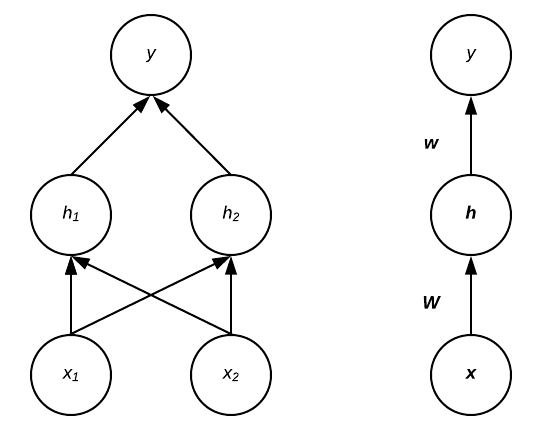
\includegraphics[scale=.4]{../img/cap7_F1NN1L.png}}
  \caption{Ejemplo de una red neuronal de 1 capa: (\textit{izquierda}). \\  Representación vectorial de las capas. (\textit{derecha})}
  \end{figure}

  \end{column}

\end{columns}

\end{frame}

\begin{frame}{Redes Neuronales - El perceptrón}

El \textit{perceptrón} corresponde a la forma más básica de una red neuronal, esta recibe un input numérico $x = (x_i)_{i=1}^n \in \R^n$ y computa la suma ponderada $u = x_1w_1 + x_2w_2 + \dots + w_nx_n + b$ donde $W = (w_i)_{i=1}^n \in \R^n$ corresponden a los \textbf{pesos} (weights) y $b \in \R$ el \textbf{sesgo} (bias). \pause 

A continuación, se aplica una función de activación $f$ y se entrega un output $h = f(u)$. \pause 
\begin{figure}[H]
  \centering
  \visible<3->{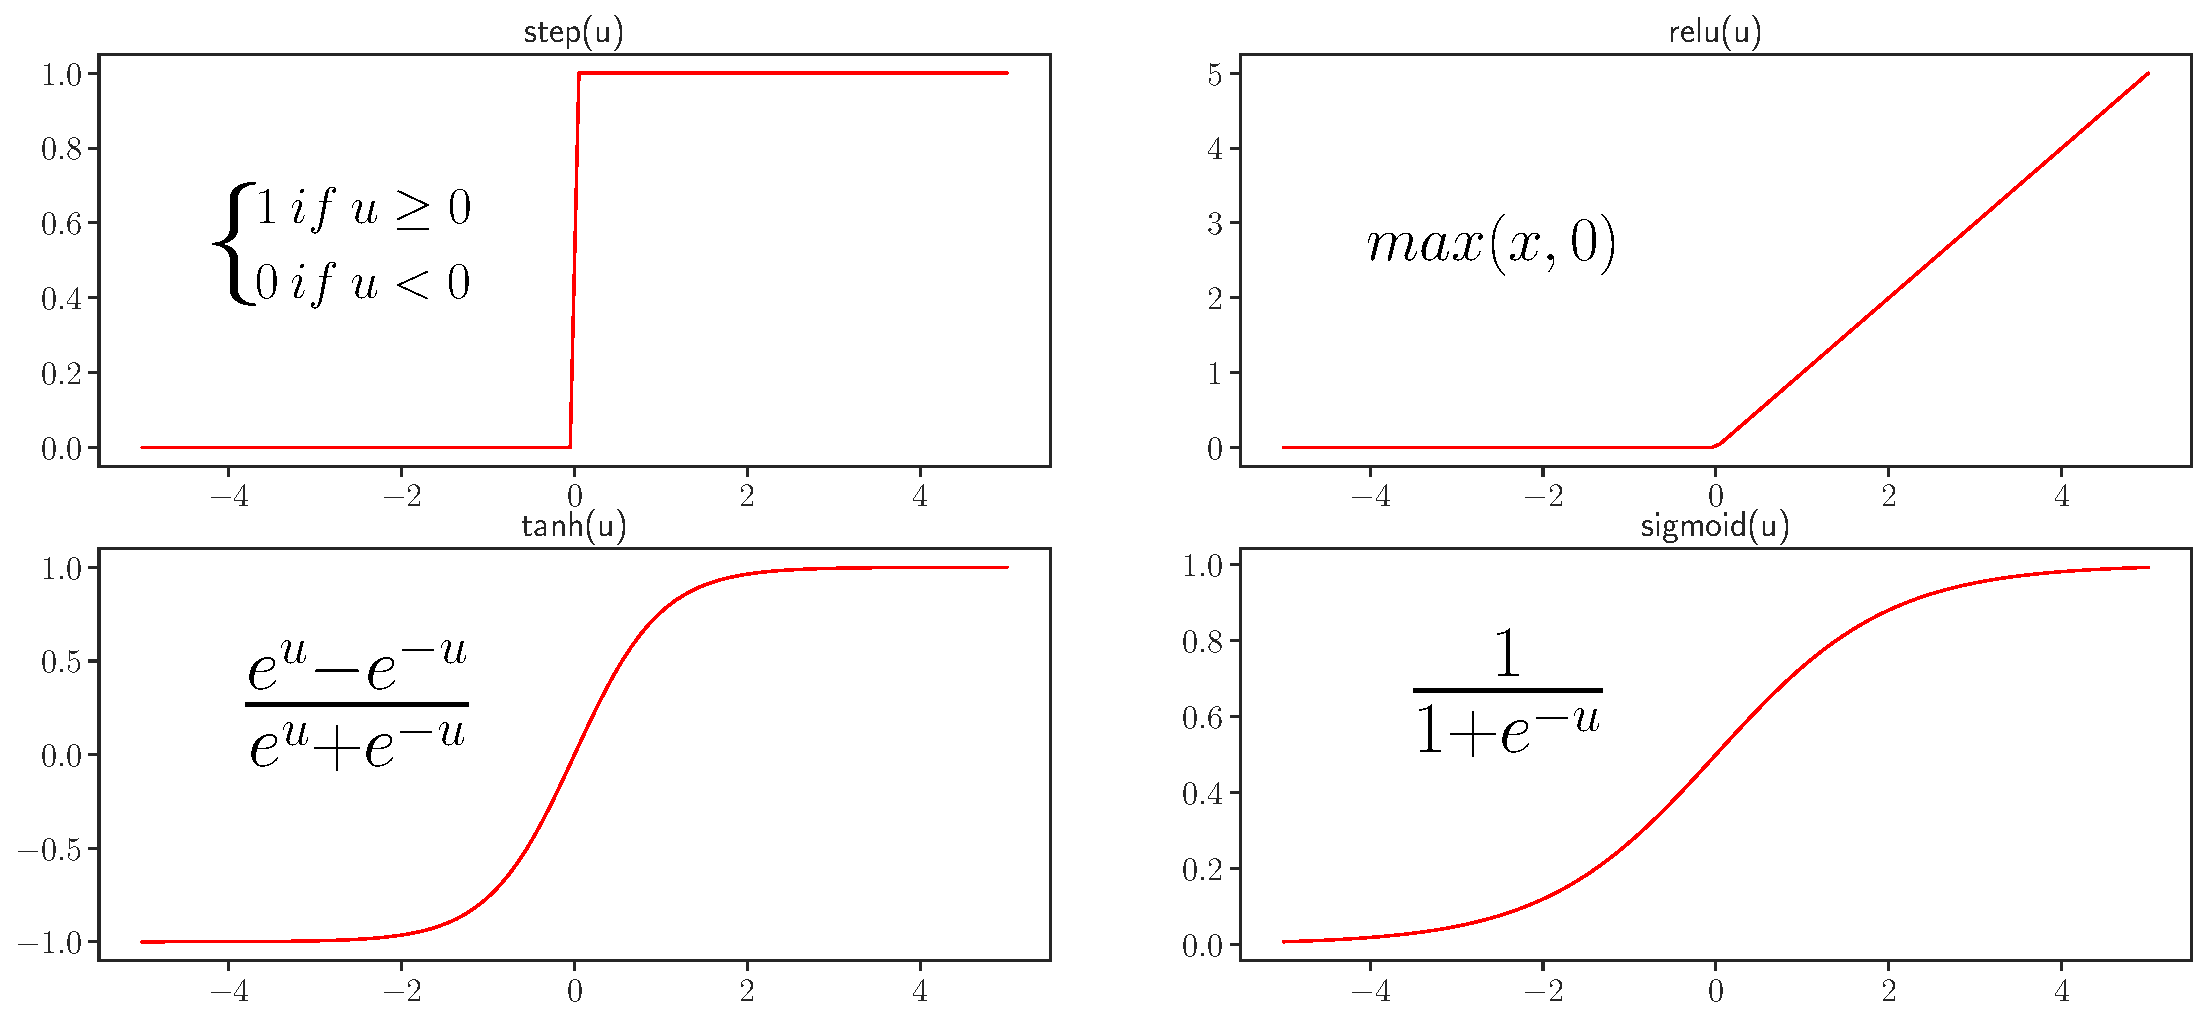
\includegraphics[scale=.3]{../img/cap5_activaciones}}
  \caption{Algunos ejemplos de funciones de activación}
\end{figure}

\end{frame}

\begin{frame}{Redes Neuronales - El perceptrón}

Veamos el siguiente ejemplo: \pause

\begin{columns}

  \begin{column}{0.7\textwidth}

  \begin{figure}[H]
    \centering
    \visible<2->{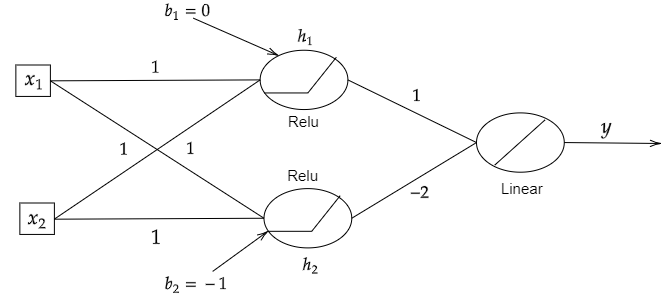
\includegraphics[scale=.3]{../img/cap7_xor}}
    \caption{Red Neuronal de 2 perceptrones para XOR}
  \end{figure}

  \end{column}

  \begin{column}{0.3\textwidth}
  
  \hspace{0.4cm} XOR operator

  \scalebox{1.3}{
  \begin{tabular}{| c  c | c |}
    \hline
    $x_1$ & $x_2$ & $y$ \\ \hline
    0 & 0 & 0 \\
    1 & 0 & 1 \\
    0 & 1 & 1 \\ 
    1 & 1 & 0 \\ \hline
  \end{tabular}
  }

  

  \end{column}

\end{columns} \pause

En su forma matricial 
$$
(h_1 , h_2) = \text{Relu} \left ( \begin{pmatrix}
x_1 & x_2  
\end{pmatrix} \begin{pmatrix}
1 &1 \\ 
 1 & 1
\end{pmatrix} + \begin{pmatrix}
0 & -1 
\end{pmatrix}\right) \hspace{0.5cm} h = \text{Relu}(xW + b)
$$
\pause
$$
y = \begin{pmatrix}
h_1 & h_2 
\end{pmatrix}\begin{pmatrix}
1 \\ 
-2 
\end{pmatrix} + (0) \hspace{0.5cm} y = hU + c
$$
Donde $U$ y $c$ corresponden al peso y bias de la última capa respectivamente. 
\textbf{¿Cómo construir el resto de operadores lógicos?}
\end{frame}

\begin{frame}{Teorema de Aproximación Universal\footnote{(Horniket al., 1989; Cybenko, 1989)} }

Un conjunto de perceptrones conectados unos con otros en secuencia forman arquitecturas capaces de resolver problemas más complejos.  \pause

Bajo el contexto de una red de múltiples perceptrones con una sola capa escondida, se tiene el siguiente resultado \pause

\begin{theorem}[UAT - Ancho arbitrario]

Sea $f^{*}$ una función objetivo Borel Medible (por ejemplo $f^{*}:[0,1]^k \rightarrow [0,1]$ continua con $k \in \N$) y sea f una función de activación no polinomial acotada, entonces para todo $\epsilon > 0$ existen $W,b,U$ definidas como antes tales que 
\[
F(x) = f(xW+b)U, \quad 
|F(x)-f^{*}(x)|<\epsilon \quad \forall x \in Dom(f^{*}) 
\]
\end{theorem} \pause
En palabras simples, con una cantidad suficiente de perceptrones, es posible aproximar una función objetivo razonable tan finamente como se desee. 
\end{frame}

\begin{frame}{Redes Neuronales - Arquitectura}

Ya vimos que es posible aproximar funciones con el uso del UAT, el principal problema es que la red podría no necesariamente 'aprender' la función en si, y tampoco asegura una cota para la cantidad de neuronas necesarias. Es por esto que surge la necesidad de arquitecturas más complejas, es decir, con mayor cantidad de capas (mayor profundidad). \pause

\begin{figure}[H]
  \centering
  \visible<2->{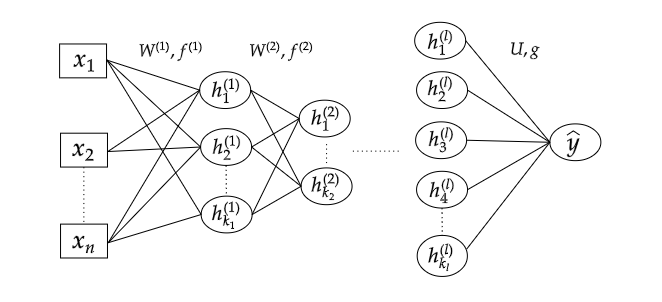
\includegraphics[scale=.3]{../img/cap7_red}}
  \caption{Una red con mayor profundidad}
\end{figure}

\pause 

Utilizaremos la siguiente notación 
\begin{equation}
h^{(k)} = f^{(k)}(h^{(k-1)}W^{(k)} + b^{(k)}) \hspace{0.3cm} \forall k \in \{1 ,\dots, l\}, \quad h^{(0)}=x
\end{equation}
\begin{equation}
\hat{y} = g(h^{(l)}U + c)
\end{equation}

Donde $g$ es la función aplicada en la capa de output y es la que define la $\textbf{unidad de output}$

\end{frame}

\section{Función de costos y unidades de output}

\begin{frame}{Función de costos}
Una de las principales diferencias entre los modelos lineales antes vistos y una red neuronal, es que el uso de ciertas funciones de activación hacen que la función de costos \textbf{no sea convexa}, esto hace que el entrenamiento realizado en base a descenso de gradiente no entregue garantías de que se alcanzará el óptimo global, o una buena solución en términos generales, ya que el algoritmo podría estancarse en un optimo local que entregue resultados pobres. \pause 
\vspace{0.2cm}

Así, para la mayor parte de los problemas a los que se enfrenta una red, nos gustaría que el modelo paramétrico defina una distribución $p(y|\bm{x}; \bm{\theta})$ y estimar los parámetros óptimos mediante máxima verosimilitud. \pause

La \textbf{función de costos} que utilizaremos entonces será la entropía cruzada (cross-entropy) definida como \pause 

\begin{equation*}
J(\bm{\theta}) = -\E_{\bm{x},\bm{y}\sim \hat{p}_{\textrm{data}}}(\textrm{log}\; p_{\textrm{modelo}}(\bm{y}|\bm{x}))
\end{equation*}


\end{frame}
     
\begin{frame}{Unidad de output}

La elección de la \textbf{Unidad de output} definirá la forma que toma la función de costos, algunos ejemplos 
\begin{enumerate}
  \item Unidad de output lineal $\hat{\bm{y}} = h^{(l)}U + c$ \pause

  Útil para cuando se busca retornar la media de una distribución Gaussiana condicional $p(\bm{y}|\bm{x}) = \mathcal{N}(\bm{y}|\hat{\bm{y}};\bm{I})$, el problema de maximizar la log-verosimilitud será equivalente minimizar el error cuadrático medio. \pause

  \item Unidad de output sigmoidal $\hat{{y}} = \text{sig}(h^{(l)}U + c)$ \pause

  Este se utiliza para problemas de clasificación binaria, cuyo output es $P(y=1|\bm{x})$ o la probabilidad de pertenecer a la clase 1. \pause

  \item Unidad de output softmax $\hat{{y}} = \text{softmax}(h^{(l)}U + c)$ \pause 

  Es una generalización de la función sigmoidal definida como 
  \begin{equation*}
  \text{softmax}(z)_i = \frac{e^{z_i}}{\sum_{j}e^{z_j}}
  \end{equation*}
  y es útil para el caso de clasificación multiclase. 
  %Se podrían agregar propiedades como estabilidad numérica producto de invarianza a la adición 
\end{enumerate}

\end{frame}

\begin{frame}
  \titlepage
\end{frame}


%Quitar de comentarios apenas se agregue alguna referencia 
%\bibliography{../capitulos/referencias} %Bibliografía
%\bibliographystyle{apacite}
\end{document} 